\documentclass[bachelor, och, labwork]{shiza}

\usepackage[utf8]{inputenc}
\usepackage{graphicx}

\usepackage[sort,compress]{cite}
\usepackage{amsmath}
\usepackage{amssymb}
\usepackage{amsthm}
\usepackage{fancyvrb}
\usepackage{longtable}
\usepackage{array}
\usepackage[english,russian]{babel}
\usepackage{minted}

\usepackage{tempora}


% \usepackage[colorlinks=false]{hyperref}


\newcommand{\eqdef}{\stackrel {\rm def}{=}}


\begin{document}

\title{Алгоритмы алгебры и теории чисел}

\course{4}

\group{431}

\napravlenie{10.05.01 "--- Компьютерная безопасность}


\author{Никитина Арсения Владимировича}


\satitle{доцент}
\saname{А.\,С.\,Гераськин}


\date{2022}

\maketitle

% Включение нумерации рисунков, формул и таблиц по разделам
% (по умолчанию - нумерация сквозная)
% (допускается оба вида нумерации)
%\secNumbering


\tableofcontents

\section{Задание лабораторной работы}

Осуществить проверку чисел на простоту с помощью теста на основе малой теоремы 
Ферма.

\section{Теоретическая часть}

Согласно малой теореме Ферма, для простого числа $p$ и произвольного числа 
$a = \overline{2,p-1}$ выполняется сравнение:
\begin{center}
    $a^{p-1} \equiv 1 ~ (mod ~ p)$.
\end{center}

Это означает, что если для нечетного числа $n$ существует такое целое число
$a = \overline{2,n-1}$, что $a^{n-1} \equiv 1 ~ (mod ~ n)$, то число $n$ вероятно
является простым. Таким образом получаем следующий вероятностный алгоритм
проверки числа на простоту:

\textit{Вход:} Нечетное число $n \geq 5$.

\textit{Выход:} "Число n, вероятно, простое" или "Число n не является простым".

\begin{enumerate}
    \item Выбрать случайное целое число $a = \overline{2, n-1}$.
    \item Вычислить $r = a^{n-1} ~(mod ~ n)$.
    \item Если $r = 1$, то ответ --- "Число n, вероятно, простое", а если $r\neq 1$,
          то ответ --- "Число n не является простым".
\end{enumerate}

Стоит отметить, что тест будет давать неверные ответы для чисел Кармайкла.


\section{Практическая часть}
\subsection{Пример работы алгоритма}
\begin{figure}[H]
    \centering
    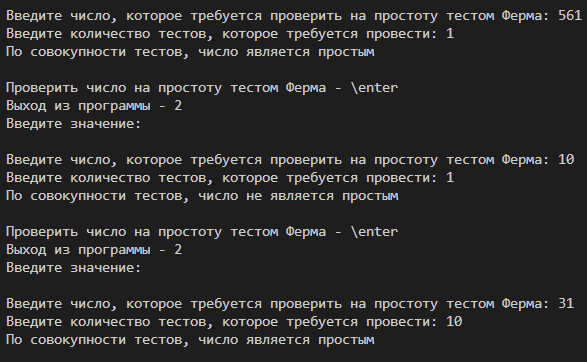
\includegraphics[width=0.8\textwidth]{pic1.png}
    \caption{}
\end{figure}

\setminted[python]{linenos,breaklines=true, fontsize=\small, style=bw}
    \subsection{Код программы, реализующей рассмотренный алгоритм}
        \inputminted{python}{lab4.py}

\end{document}